\paragraph{Question 1}
La complexité est de $O(m(n+m))=O(n^4)$ car~:
\begin{itemize}
\item La taille de la coupe augmente d'un sommet à chaque tour, donc
il nous faut $m$ étapes pour trouver la coupe maximum.
\item À chaque tour, on rajoute un également toutes les arêtes
incidentes au sommet rajouté.
\end{itemize}

\paragraph{Question 2}
Montrons que le taux d'approximation est de 2~:
\begin{proof}Soit $(Y_1,Y_2)$ la coupe approximatif. Supposons pour $\Gamma(x)$ l'ensemble des sommets voisins d'un sommet x~:

$\exists x \in Y_1 \text{ | } \Gamma(x) \cap Y_1 > \Gamma(x) \cap Y_2$

Dans un tel cas le déplacement du sommet x dans $Y_2$ augmenterai la valeur de la coupe, donc l'algorithme approché ne l'aurait jamais gardé dans $Y_1$. Notre supposition est donc absurde. Nous avions au contraire~:

$\forall x \in Y_1 \text{ | } \Gamma(x) \cap Y_1 \leq \Gamma(x) \cap Y_2$

Le même raisonnement tient pour les sommets de $Y_2$. Or la somme des degrés est égale à $2|E|$ donc~:

\begin{eqnarray*}
2|E| &=& \Sigma_{x \in Y_1}|\Gamma(x)|  + \Sigma_{x' \in Y_2}|\Gamma(x')| \\
	 &=& \Sigma_{x \in Y_1}[|(\Gamma(x)\cap{} Y_1)|\cup|(\Gamma(x)\cap{}Y_2)|] +
	 	 \Sigma_{x' \in Y_2}[|(\Gamma(x')\cap{} Y_1)|\cup|(\Gamma(x')\cap{}Y_2)|] \\
	 &=& \Sigma_{(x,x') \in (Y_1,Y_2)} +
	 	 \Sigma_{(y,y') \in (Y_2,Y_1)} + 
	 	 \Sigma_{(z,z') \in (Y_1,Y_1)} +
	 	 \Sigma_{(t,t') \in (Y_2,Y_2)} 
\end{eqnarray*}

Or $\Sigma_{(x,x') \in (Y_1,Y_2)} \geq \Sigma_{(z,z') \in (Y_1,Y_1)}$ et $\Sigma_{(y,y') \in (Y_2,Y_1)} \geq \Sigma_{(t,t') \in (Y_2,Y_2)}$ nous avons~:

\begin{eqnarray*}
\Sigma_{(x,x') \in (Y_1,Y_2)} + \Sigma_{(y,y') \in (Y_2,Y_1)} &\geq& |E| \\
\Rightarrow |(Y_1, Y_2)| &\geq& \frac{|E|}{2}
\end{eqnarray*}

Globalement au moins la moité des arrêtes doivent donc traverser la coupe approximatif. De plus la coupe optimale est évidement borné par $|E|$, donc $\frac{(Y_1,Y_2)}{(Y_1,Y_2)^*} \geq \frac{|E|}{2|E|}$, soit $\frac{(Y_1,Y_2)^*}{(Y_1,Y_2)} \geq 2$, \emph{quod erat demonstrandum}.
\end{proof}

\paragraph{Question 3}

Prenons le graphe figure \ref{coupe_max_instance}. La coupe optimale (figure \ref{coupe_max_opt}) traverse chacun des 15 arrêtes, il suffit donc de montrer que la coupe approximatif n'en traverse que 7. 

\begin{figure}[ht]
% LEFT-HAND SIDE
\begin{minipage}[b]{0.5\linewidth}
\centering
\centering
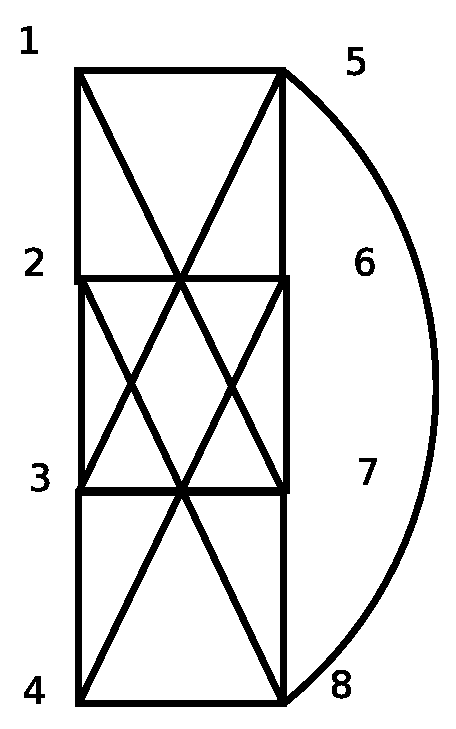
\includegraphics[width=0.4\textwidth]{../images/exo4.eps}
\caption{Instance coupe maximum.}
\label{coupe_max_instance}
\end{minipage}
% RIGHT-HAND SIDE
\hspace{0.5cm}
\begin{minipage}[b]{0.4\linewidth}
\centering
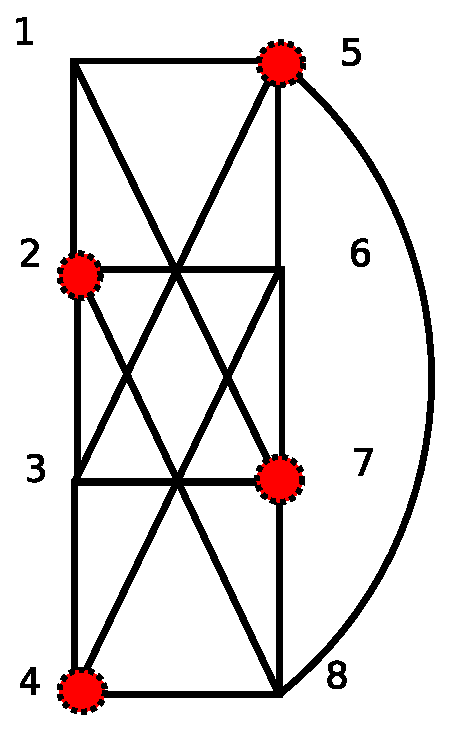
\includegraphics[width=0.5\textwidth]{../images/exo4_opt.eps}
\caption{Coupe optimale.}
\label{coupe_max_opt}
\end{minipage}
\end{figure}

\begin{figure}[h!]

\end{figure}

Les sommets sont de degré 3 ou 4
